\section{Systemablaufmodell}\label{sec:Systemablaufmodell}
\begin{figure}
  \centering
  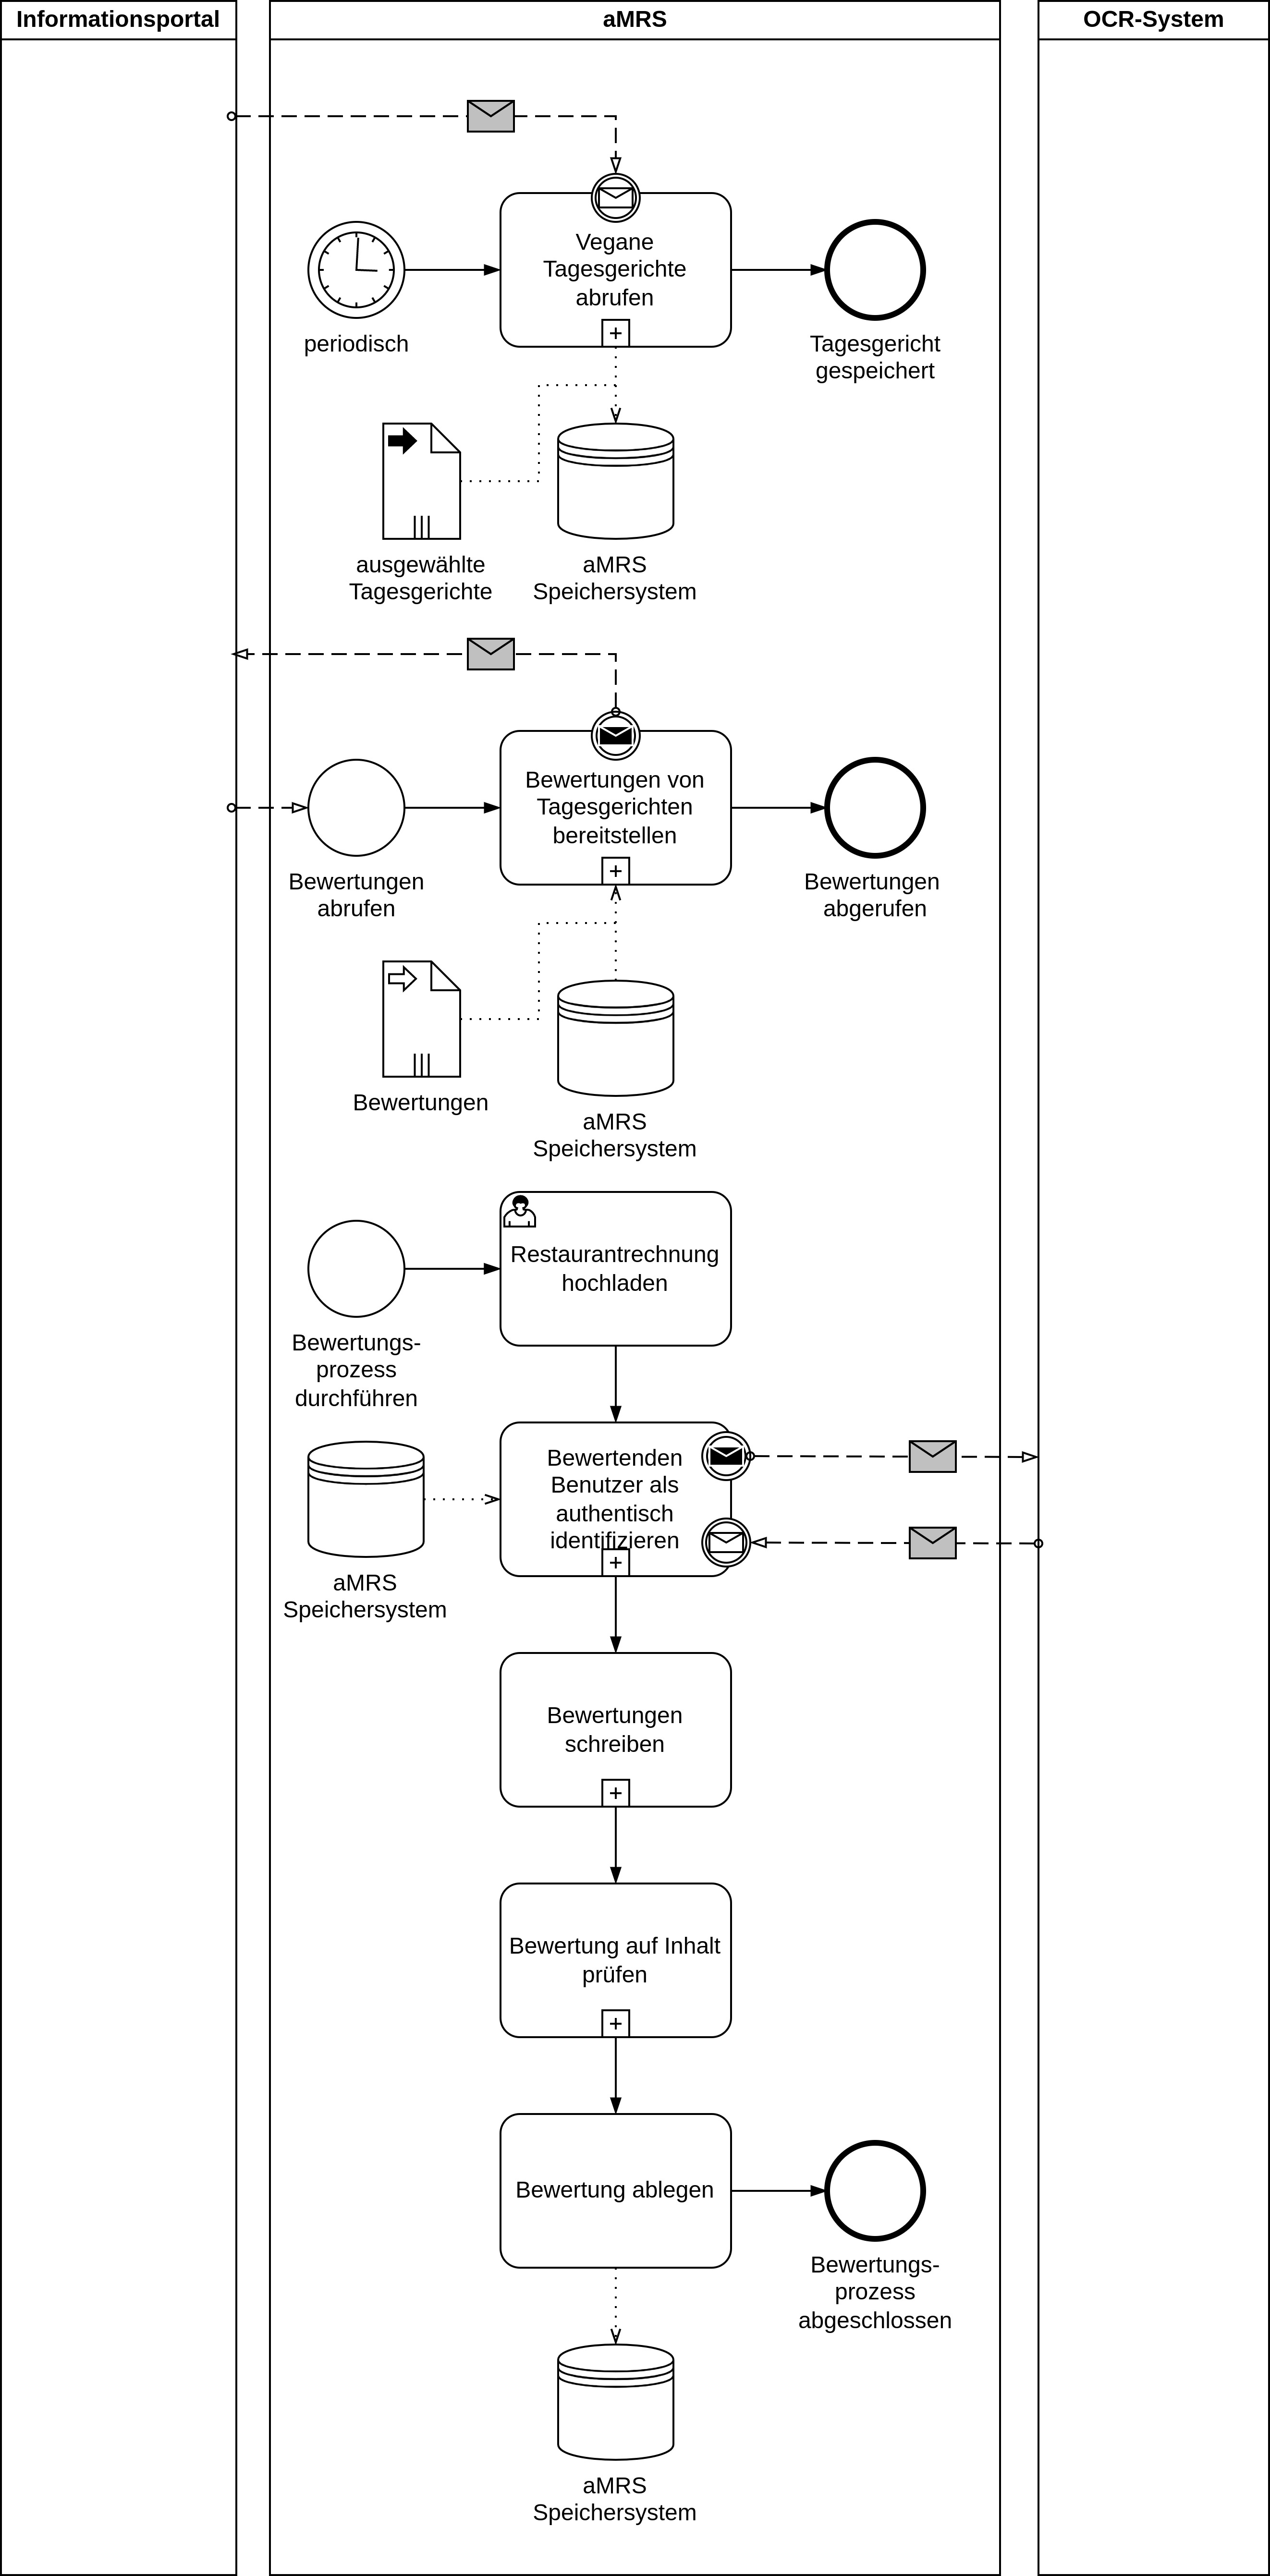
\includegraphics[height=0.765\paperheight]{Systemablaufmodell.jpg}
  \caption{Systemablaufmodell}
  \label{fig:Systemablaufmodell}
\end{figure}
% Ablauf Geschäftsmodelle
% Zusammenspiel der Systeme
% Standardablauf ohne große Abweichungen
Die in Kapitel~\ref{sec:Geschaeftsfaelle} aufgelisteten Geschäftsfälle werden nun in Abbildung~\ref{fig:Systemablaufmodell} zu einem Systemablaufmodell zusammengefügt.
Dabei wird das Zusammenspiel zwischen dem vorhandenen Informationsportal, dem zu entwickelnden System \ac{aMRS} und dem \hyperref[gls:ocr-System]{OCR-System} als externem System dargestellt.

\noindent{}Abbildung~\ref{fig:Systemablaufmodell} zeigt dabei den Standardablauf des Systems und bietet zunächst einen Überblick über die drei Hauptfunktionen des Systems.
In den fünf darauffolgenden Abbildungen (\ref{fig:VeganeTagesgerichteAbrufen}-\ref{fig:BewertungAufInhaltPruefen}) werden die einzelnen Schritte der verschiedenen Geschäftsfälle genauer betrachtet.

\begin{figure}
  \centering
  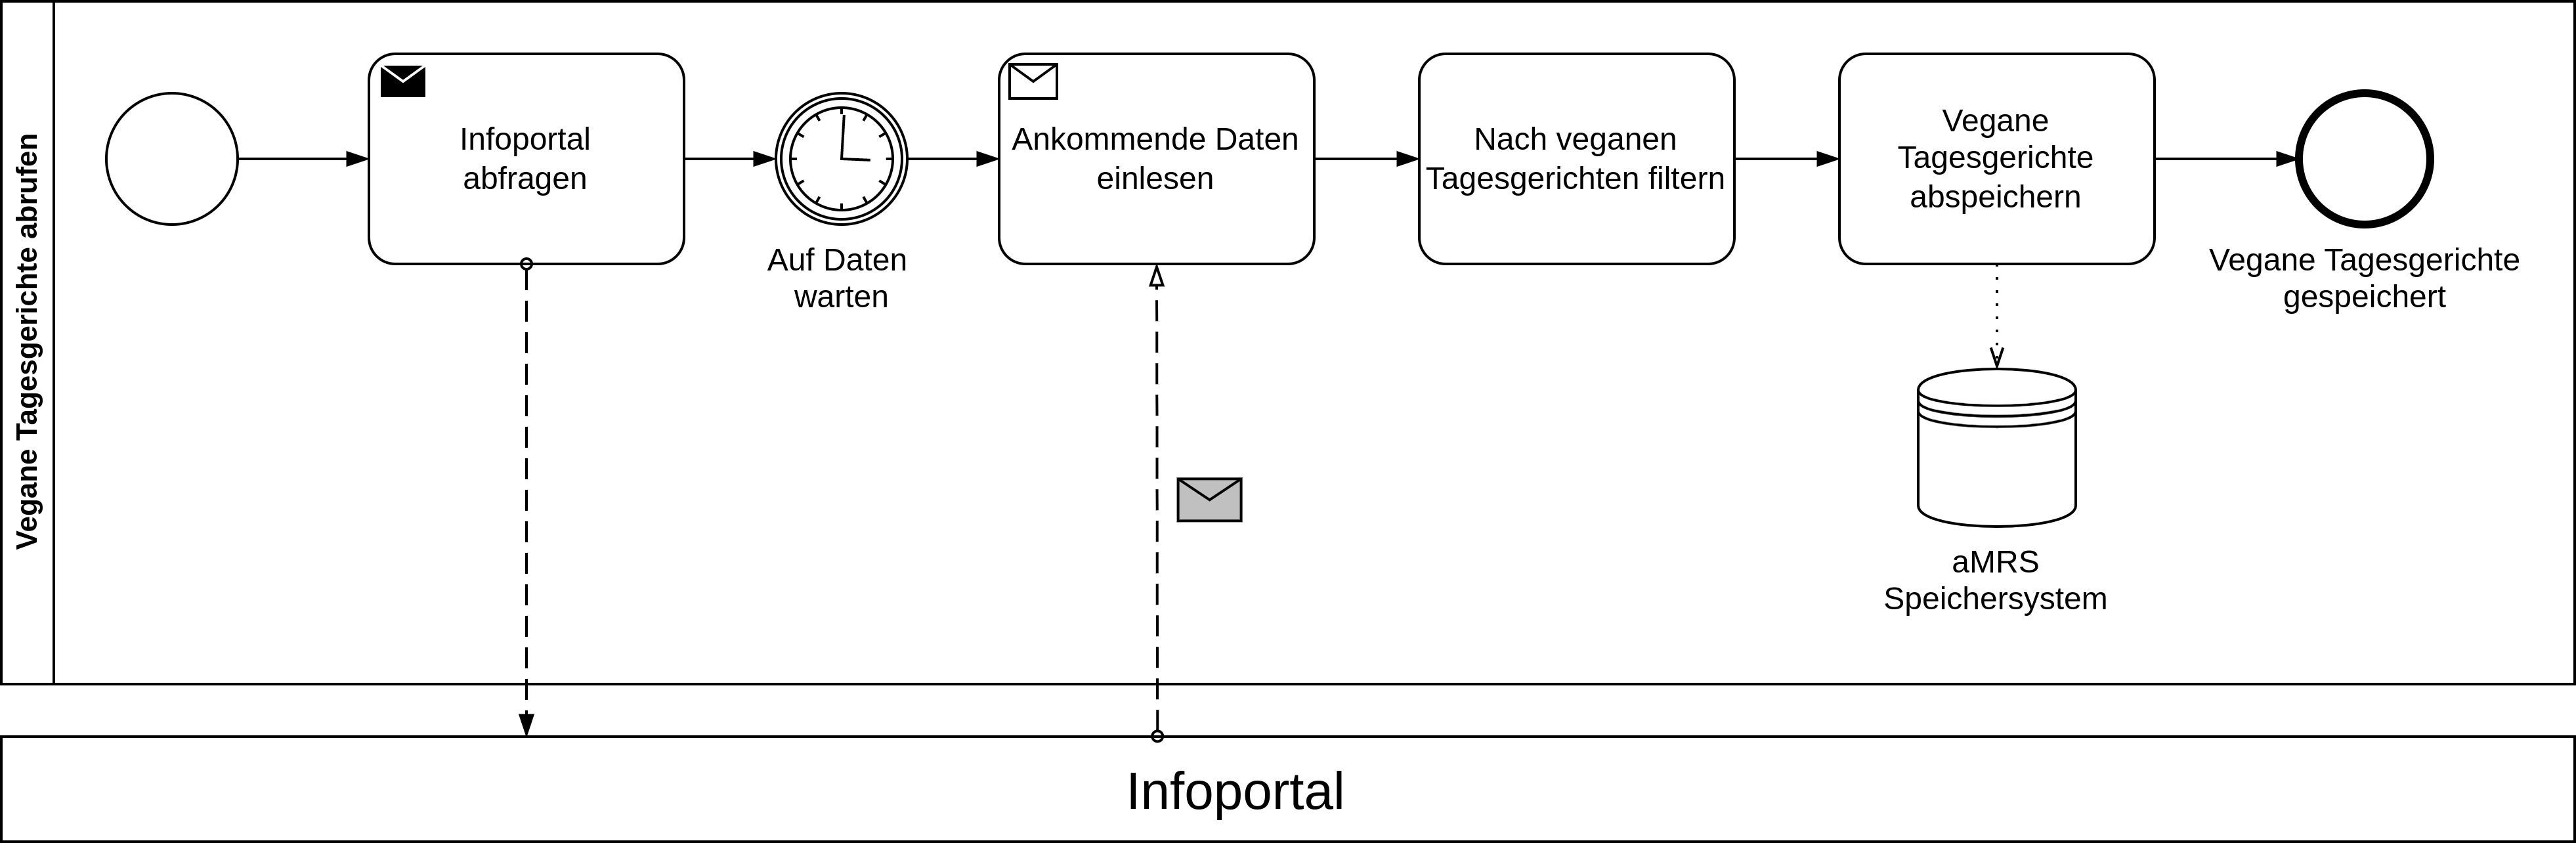
\includegraphics[width=1\linewidth]{VeganeTagesgerichteAbrufen}
  \caption{Systemablaufmodell - Vegane Tagesgerichte abrufen}
  \label{fig:VeganeTagesgerichteAbrufen}
\end{figure}
\begin{figure}
  \centering
  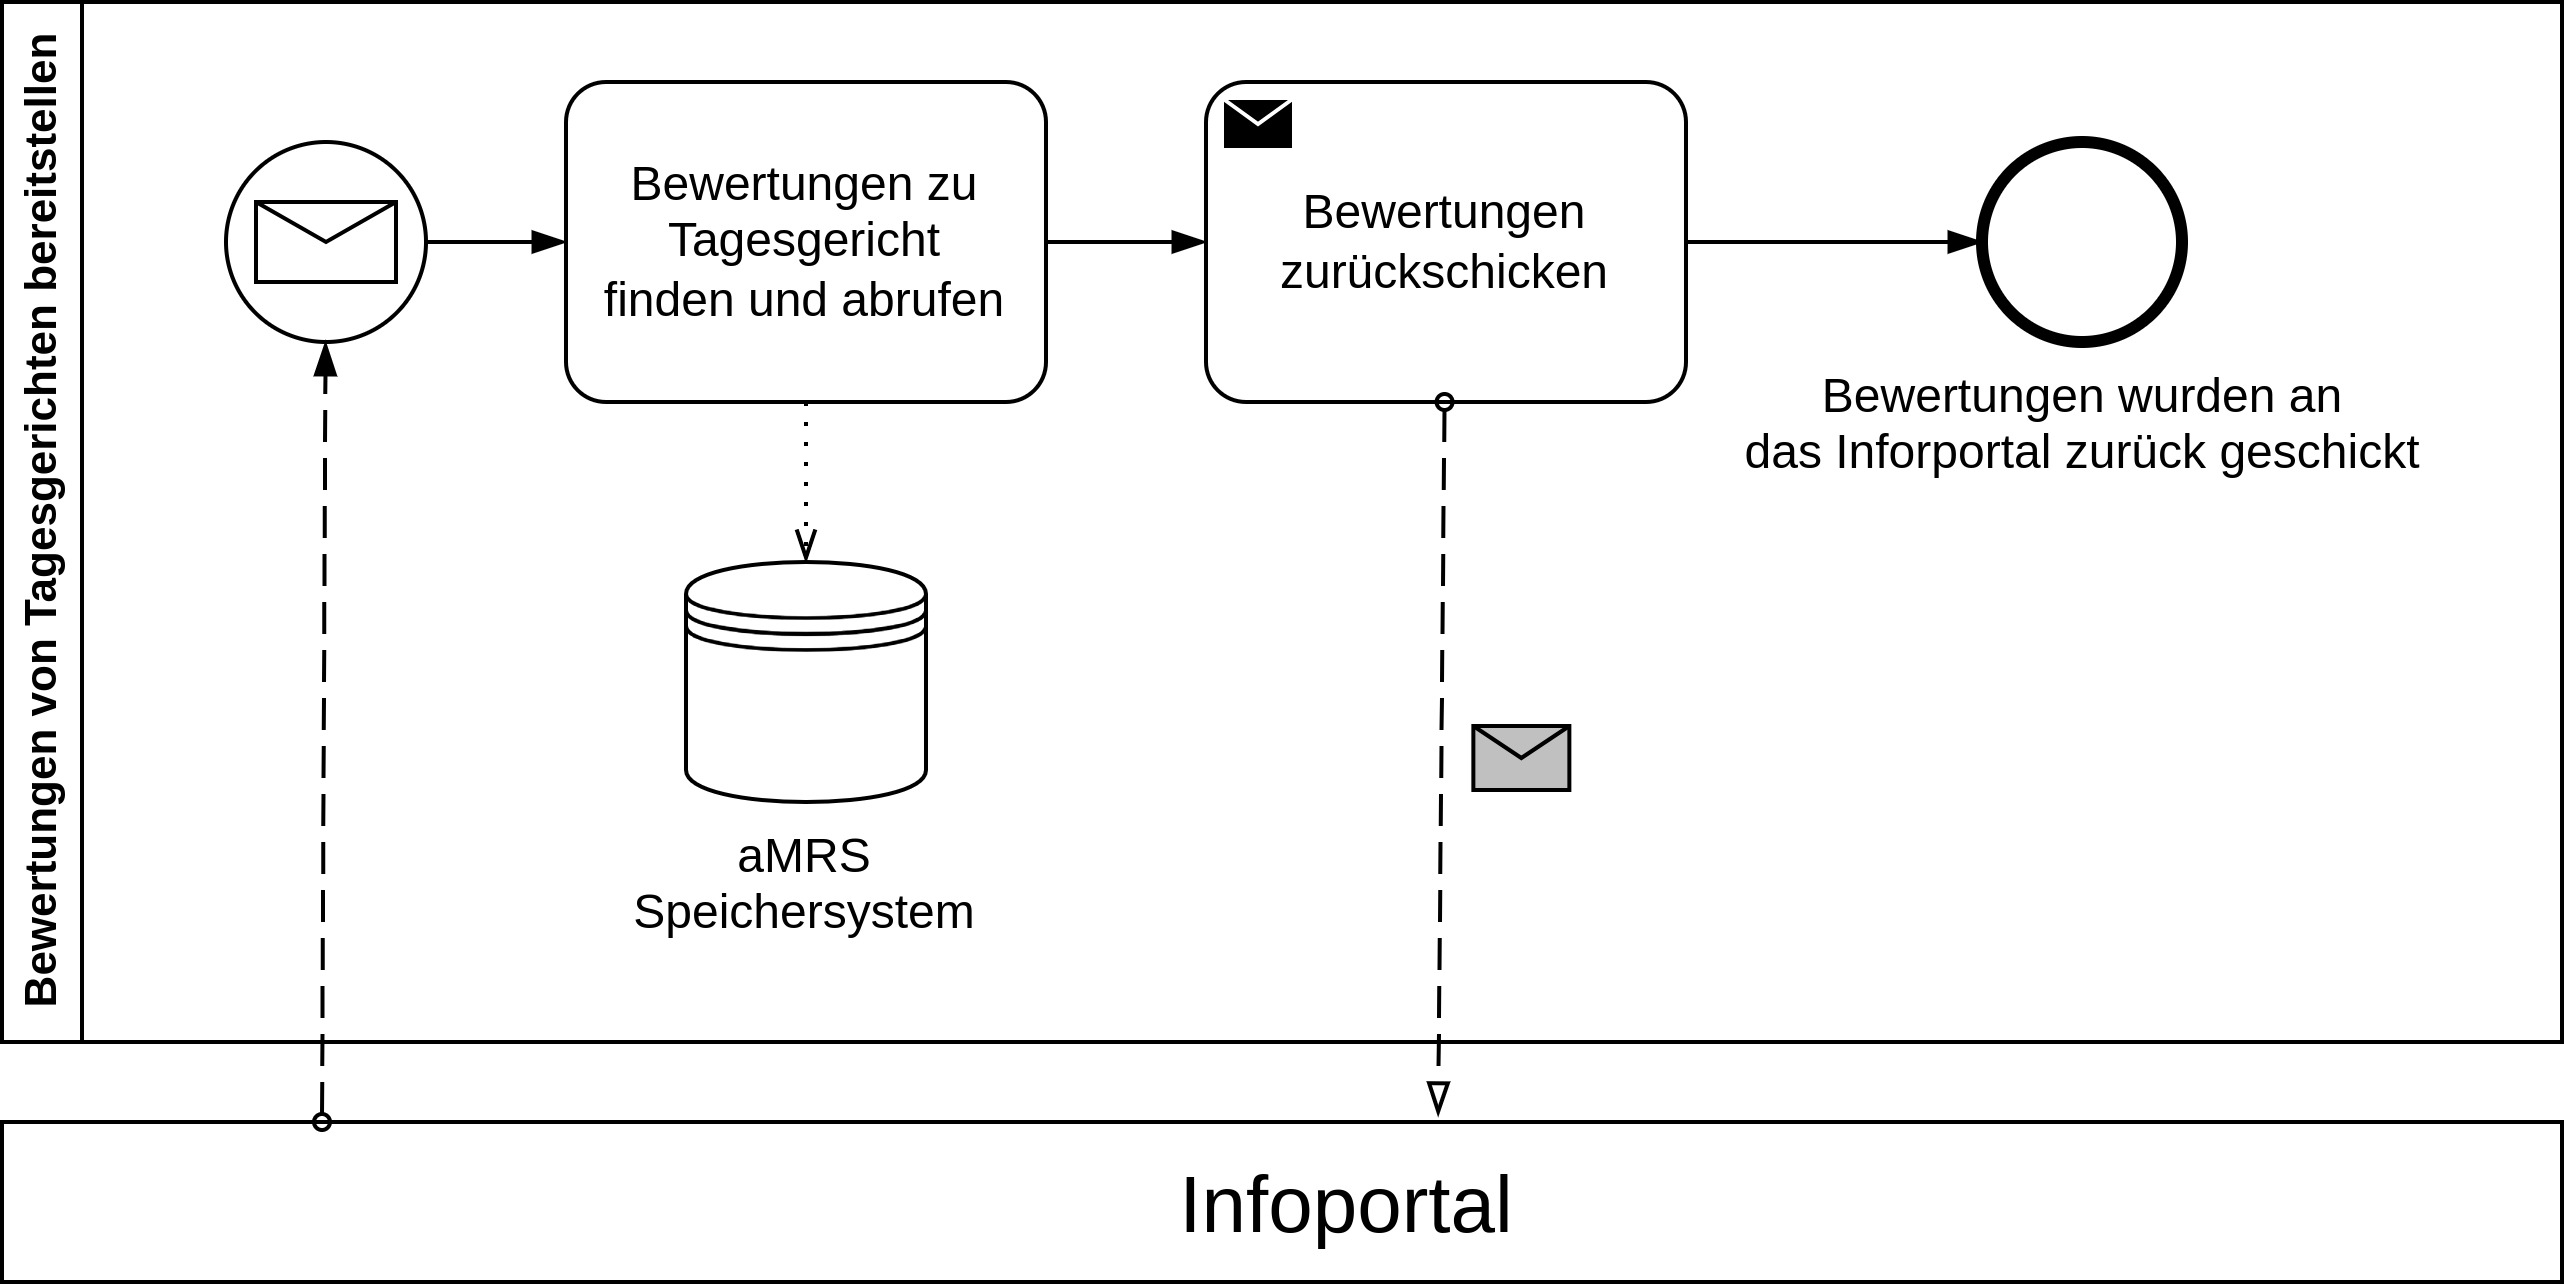
\includegraphics[width=0.8\linewidth]{BewertungenBereitstellen}
  \caption{Systemablaufmodell - Bewertungen von Tagesgerichten bereitstellen}
  \label{fig:BewertungenVonTagesgerichtenBereitstellen}
\end{figure}
\begin{figure}
  \centering
  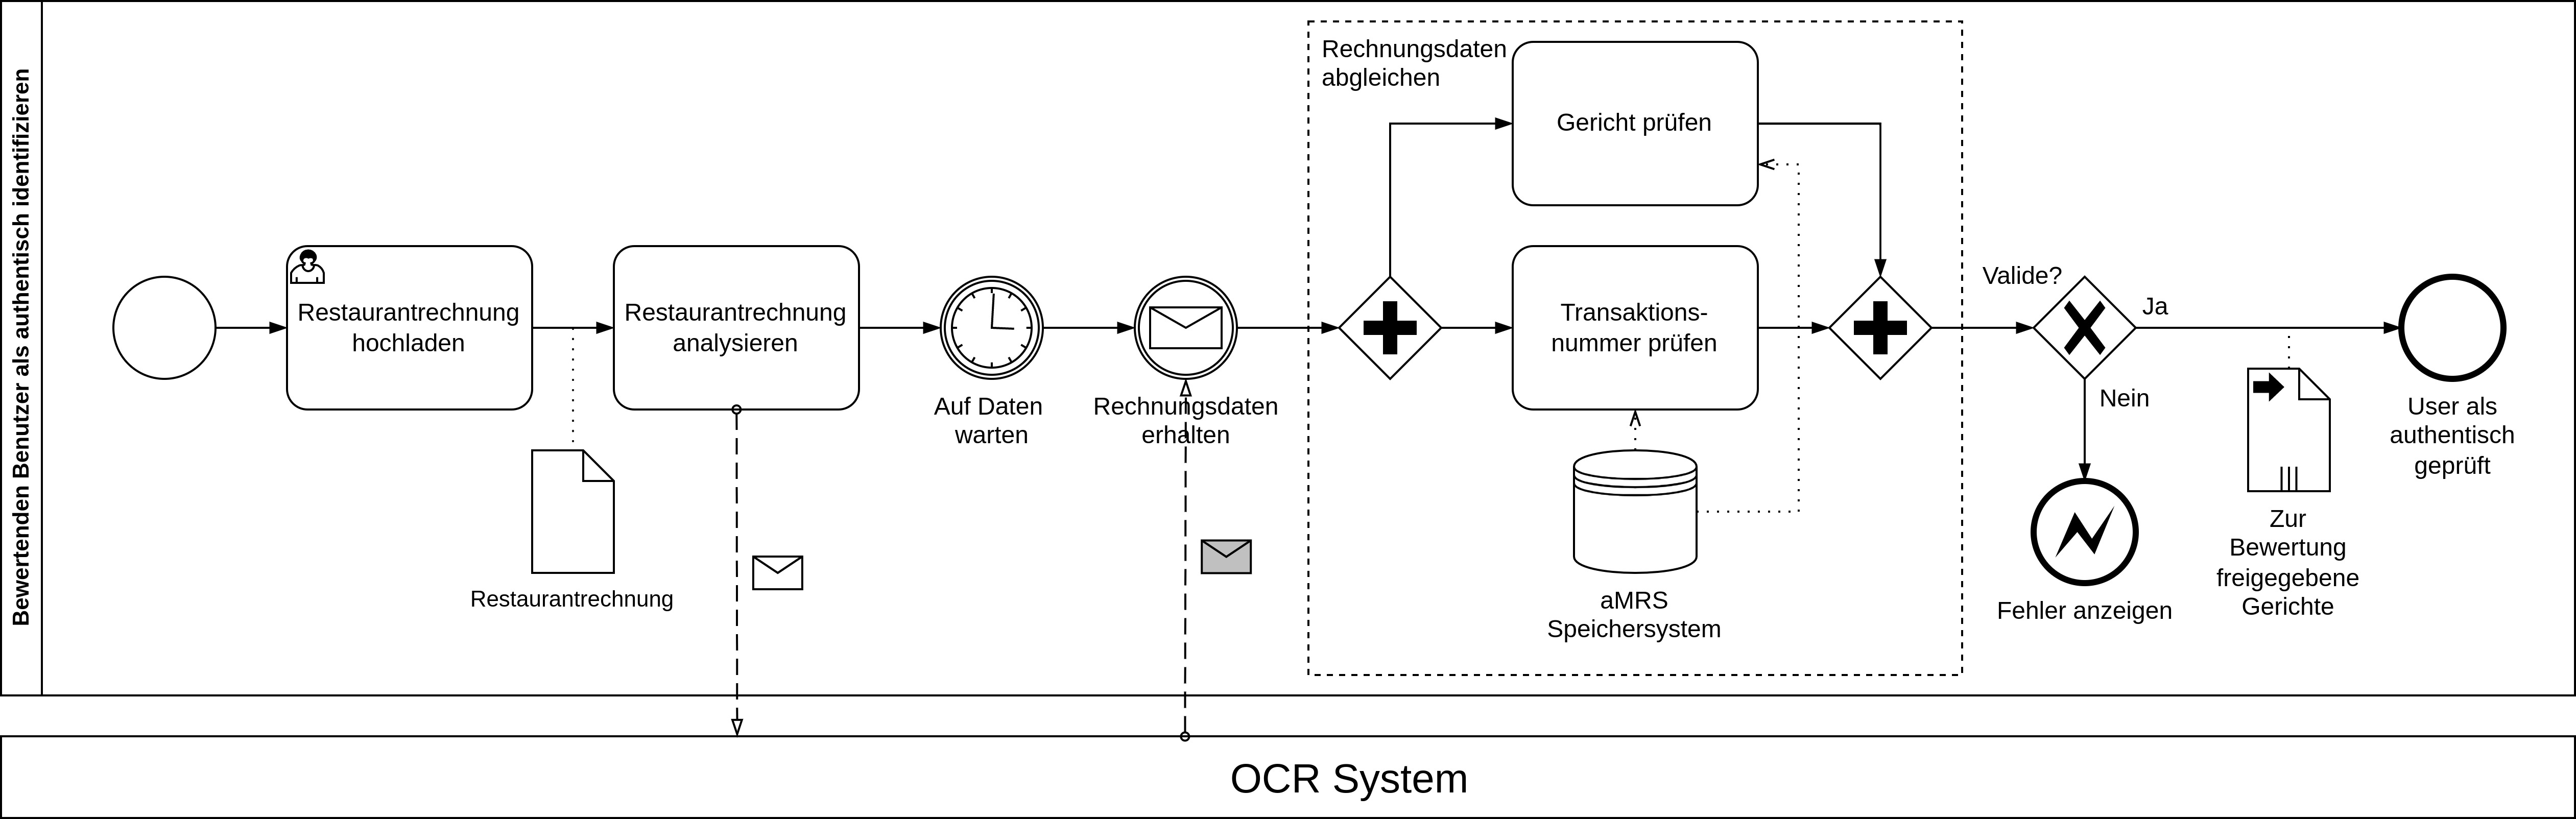
\includegraphics[width=1\linewidth]{BewertendenBenutzerAuthentisch}
  \caption{Systemablaufmodell - Bewertenden Benutzer als authentisch identifizieren}
  \label{fig:BewertendenBenutzerAlsAuthentischIdentifizieren}
\end{figure}
\begin{figure}
  \centering
  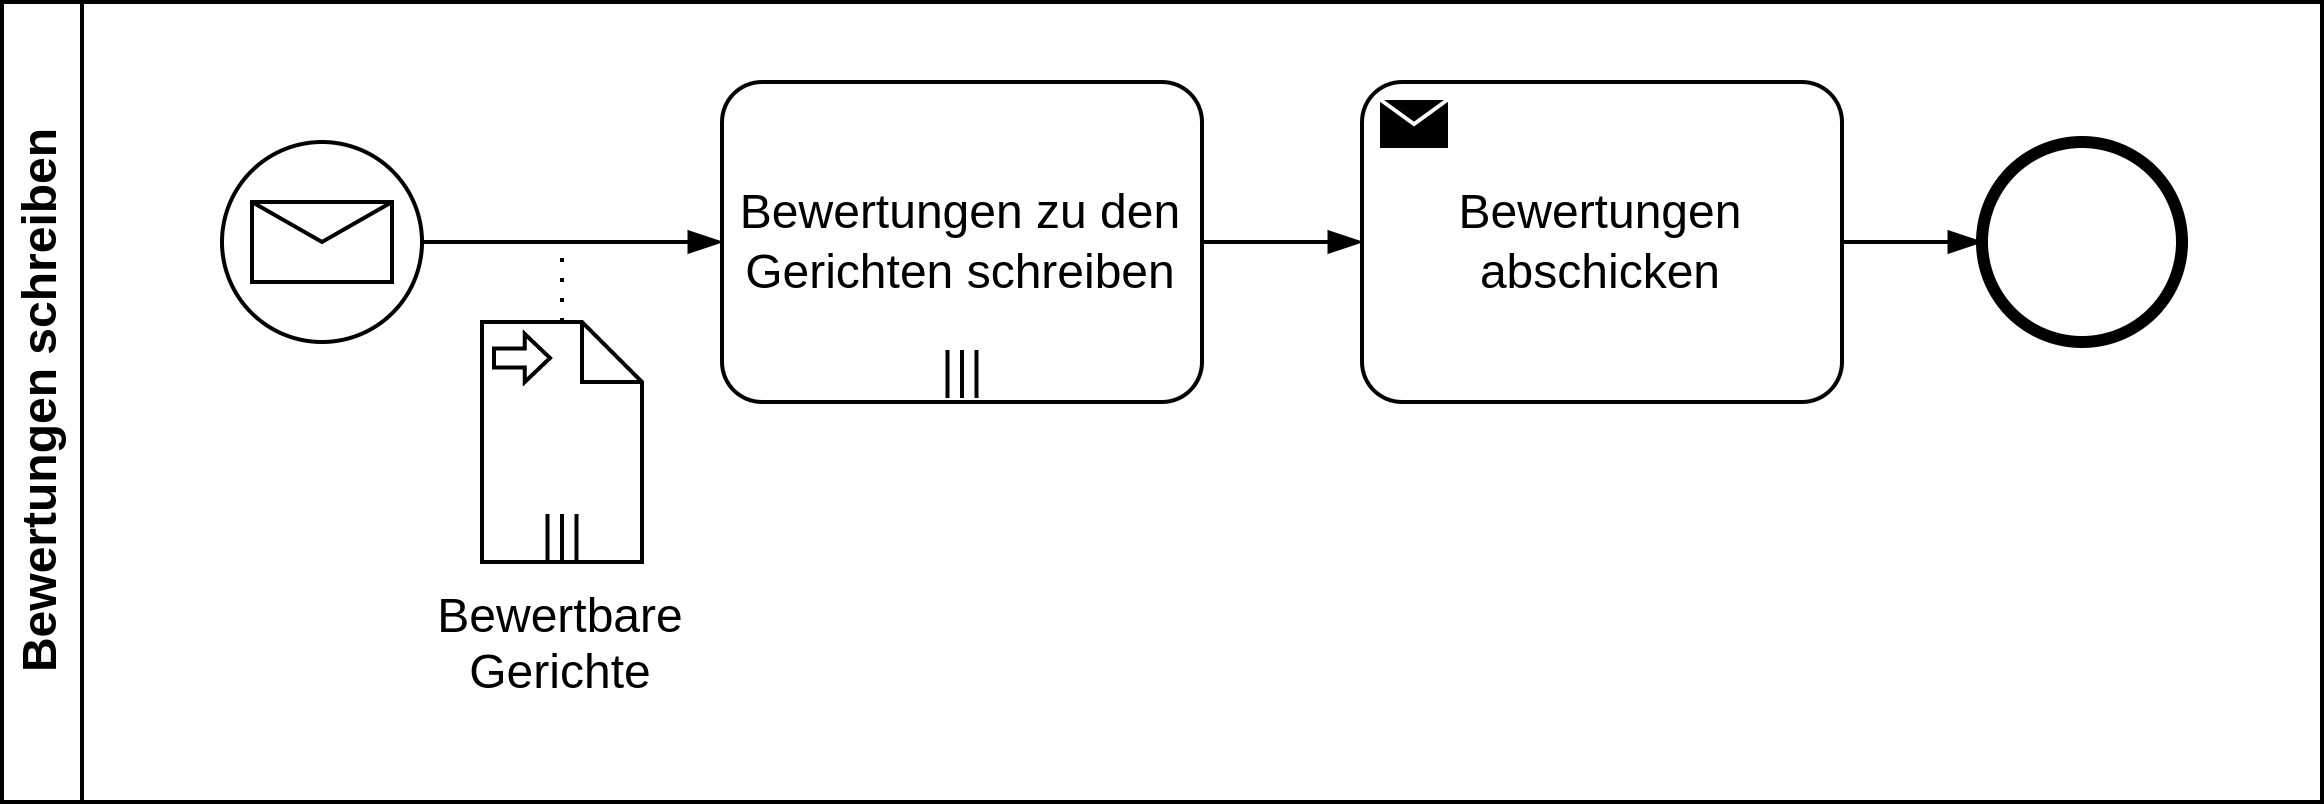
\includegraphics[width=0.9\linewidth]{BewertungSchreiben}
  \caption{Systemablaufmodell - Bewertung schreiben}
  \label{fig:BewertungSchreiben}
\end{figure}
\begin{figure}
  \centering
  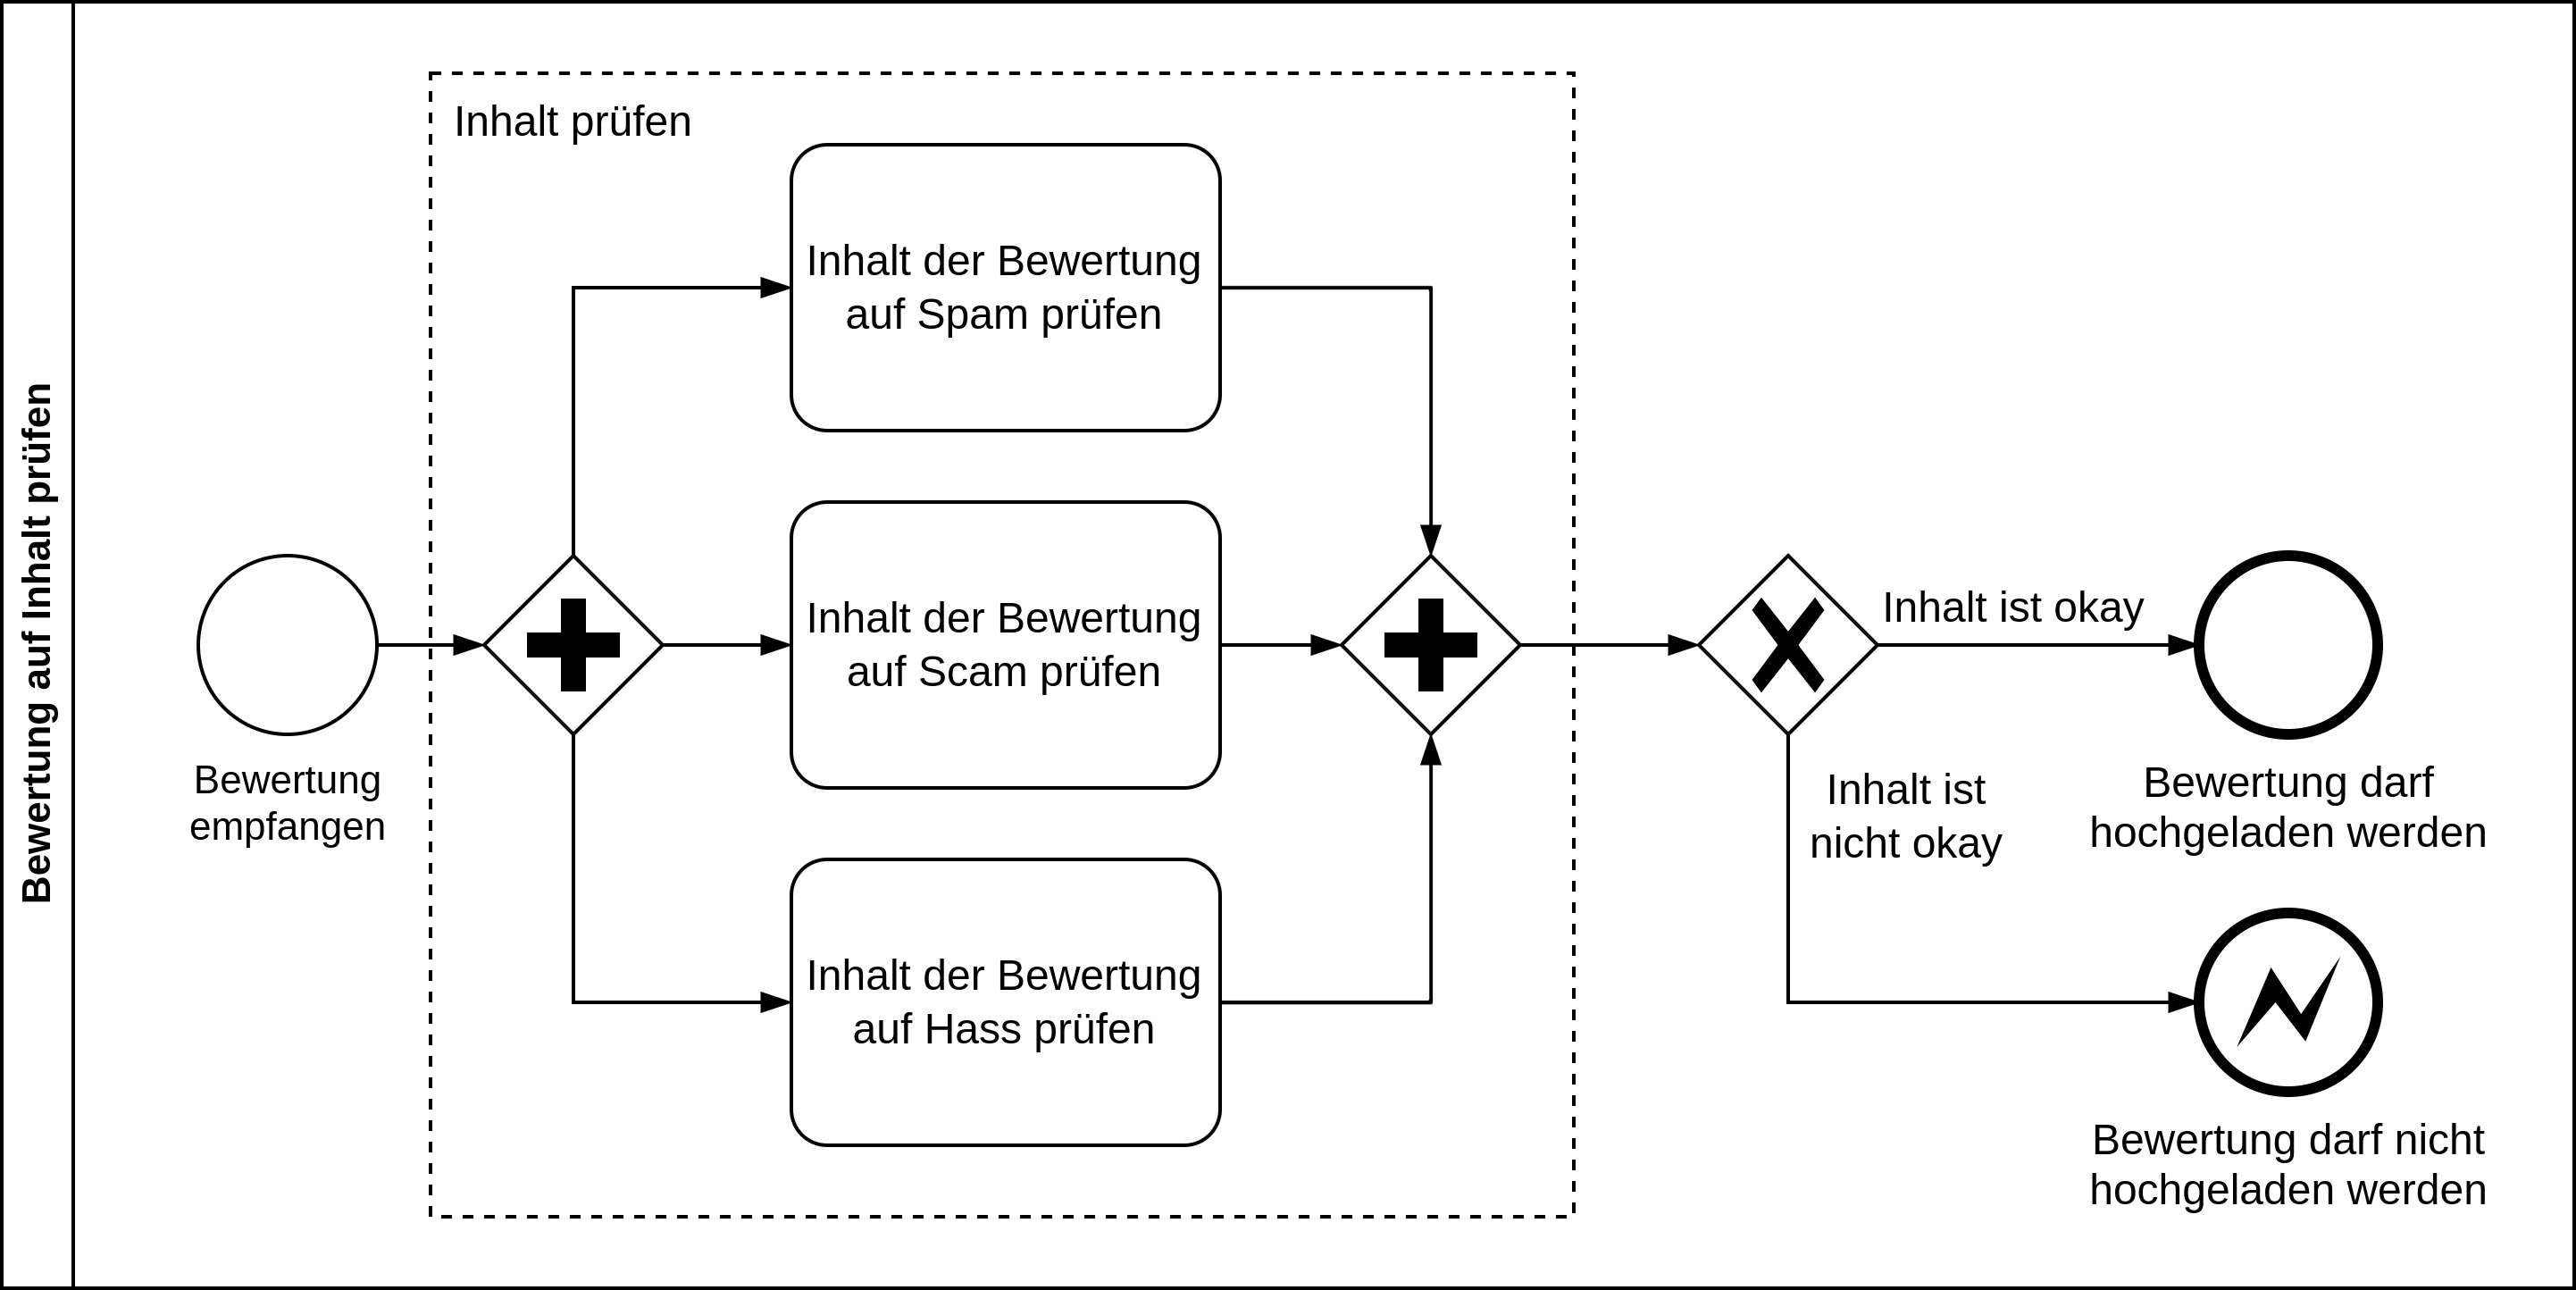
\includegraphics[width=0.9\linewidth]{BewertungInhaltPruefen}
  \caption{Systemablaufmodell - Bewertung auf Inhalt prüfen}
  \label{fig:BewertungAufInhaltPruefen}
\end{figure}